% rubber: module pdftex

\documentclass[a4paper,11pt]{article}
\usepackage[top = 1.5 in, bottom = 1 in, left = 1 in, right = 1 in]{geometry}
\usepackage[utf8]{inputenc}
\usepackage[T1]{fontenc}
\usepackage{csquotes}
\usepackage[british]{babel}
\usepackage{lmodern}
\usepackage{url}
\usepackage{color}
\usepackage{graphicx}
\usepackage{setspace}
\usepackage{pdfpages}
\usepackage{amsmath}
\usepackage[usenames,dvipsnames]{xcolor}
\usepackage{hyperref}
\hypersetup{
  colorlinks=true,
  urlcolor=Blue,
  linkcolor=Blue
}
\begin{document}
\title{Mini-Java compiler}
\author{Laura Leppänen \\ Compiler Project 2013}
\date{\today}
\maketitle
\thispagestyle{empty}

\tableofcontents
\onehalfspacing

\newpage
\setcounter{page}{1}

\section{The Mini-Java language}

\subsection{Token patterns}

Defined using regular expressions with Java style character classes. These token groups correspond to token classes used in the implementation.

\begin{description}
\item[Identifiers] $\backslash\text{p\{IsAlphabetic\}} [ \backslash\text{p\{IsAlphabetic\}}\backslash\text{p\{IsDigit\}\_ } ]^{*}$ \\ \emph{Except simple types and keywords.}
\item[Integer literals] $\backslash\text{p\{IsDigit\}}^{+}$ \\ \emph{Note that this allows literals with leading zeros such as 00115. Literals like this would be interpreted as octal numbers in Java. This implementation interprets these literals as decimal integers, so 00115 would be decimal integer 115.}
\item[Simple type] int | boolean | void
\item[Keyword] class | public | static | main | extends | assert | if | else | \\ while | System | out | println | return | new | length | this | true | false
\item[Operator] \&\& | || | < | > | == | + | - | *  | / | \% | = | !
\item[Punctuation] \{ | \} | [ | ] | ( | ) | $\backslash$. | ; | ,
\end{description}

\subsection{Modified grammar for recursive descent parsing (non-LL(1))}

In the grammar below, I have solved operator precedences by making a separate production rule for each level of operator precedence. This is very easy to implement in the case of Mini-Java especially since all the defined binary operators are left-associative and there is only one unary operator.\footnote{Note: A program example on the course's grammar page also uses a unary minus operator, but this is not reflected in the grammar that was given, so I have left it out.} Different solutions to the operator precedence problem are described on Theodore Norvell's website \url{http://www.engr.mun.ca/~theo/Misc/exp_parsing.htm}. I used the so called ''classic solution'' described on Norvell's site a basis for my implementation. Norvell does not give a source for the algorithm but mentions that Niklaus Wirth used it in his Pascal compilers. 

A look-ahead of more than one token is needed e.g. when the parser sees an identifier in the input and is trying to parse a statement. In this case the result could be a local variable declaration for either a user defined type or an array of a user defined type or a statement that starts with an expression that begins with a variable reference.

\begin{verbatim}
<program>              ::= <main class> <class declaration list>
<main class>           ::= "class" <identifier> "{" "public" "static" "void" "main"
                           "(" ")" "{" <statement list> "}" "}"
<class declaration>    ::= "class" <identifier> <optional inheritance> "{"
                           <declaration list> "}"
<optional inheritance> ::= "extends" <identifier>
                        |  epsilon
<declaration>          ::= <variable declaration>
                        |  <method declaration>

<class declaration list> ::= <class declaration> <class declaration list>
                          |  epsilon
<declaration list>       ::= <declaration> <declaration list>
                          |  epsilon
<statement list>         ::= <statement> <statement list>
                          |  epsilon

<method declaration>   ::= "public" <type> <identifier> "(" <opt formals> ")"
                           "{" <statement list> "}"
<opt formals>          ::= <type> <identifier> <formals list>
                        |  epsilon
<formals list>         ::= "," <type> <identifier> <formals list>
                        |  epsilon
<variable declaration> ::= <type> <identifier> ";"
<type>                 ::= <simple type> <opt brackets>
<simple type>          ::= "int" | "boolean" | "void" | <type identifier>
<opt brackets>         ::= "[" "]" | epsilon
<type identifier>      ::= <identifier>

<statement>      ::= "assert" "(" <expr> ")" ";"
                  |  <local variable declaration>
                  |  "{" <statement list> "}"
                  |  "if" "(" <expr> ")" <statement> <opt else>
                  |  "while" "(" <expr> ")" <statement>
                  |  "System" "." "out" "." "println" "(" <expr> ")" ";"
                  |  "return" <expr> ";"
                  |  <expr> <opt assignment> ";"
<opt else>       ::= "else" <statement> | epsilon
<opt assignment> ::= "=" <expr> | epsilon
<local variable declaration> ::= <variable declaration>

<expr> ::= <or-operand> <or-operand-list>
<or-operand> ::= <and-operand> <and-operand-list>
<and-operand> ::= <eq-operand> <eq-operand-list>
<eq-operand>  ::= <neq-operand> <neq-operand-list>
<neq-operand> ::= <add-operand> <add-operand-list>
<add-operand> ::= <mult-operand> <mult-operand-list>
<mult-operand> ::= "!" <term>
                |  <term>

<or-operand-list> ::= "||" <or-operand> <or-operand-list>
                   |  epsilon
<and-operand-list> ::= "&&" <and-operand> <and-operand-list>
                    |  epsilon
<eq-operand-list> ::= "==" <eq-operand> <eq-operand-list>
                   |  epsilon
<neq-operand-list> ::= "<" <neq-operand> <neq-operand-list>
                    |  ">" <neq-operand> <neq-operand-list>
                    |  epsilon
<add-operand-list> ::= "+" <add-operand> <add-operand-list>
                    |  "-" <add-operand> <add-operand-list>
                    |  epsilon
<mult-operand-list> ::= "/" <mult-operand> <mult-operand-list>
                     |  "*" <mult-operand> <mult-operand-list>
                     |  "%" <mult-operand> <mult-operand-list>
                     |  epsilon

<term>    ::= "new" <new type> <opt term tail>
           |  "(" <expr> ")" <opt term tail>
           |  <identifier> <opt term tail>
           |  <integer literal> <opt term tail>
           |  "this" <opt term tail>
           |  "true" <opt term tail>
           |  "false" <opt term tail>

<new type>          ::= <simple type> "[" <expr> "]"
                     |  <type identifier> "(" ")"
<opt term tail>     ::= "[" <expr> "]" <opt term tail>
                     |  "." <method invocation> <opt term tail>
                     |  epsilon
<method invocation> ::= "length"
                     |  <identifier> "(" <opt exprs> ")"
<opt exprs>         ::= <expr list> | epsilon
<expr list>         ::= <expr> <expr list tail>
<expr list tail>    ::= "," <expr list> | epsilon

\end{verbatim}

\subsection{Abstract syntax trees}

In this section I describe the interfaces and classes implementing the abstract syntax tree representation and their relationships in the syntax tree. Due to the large number of classes the syntax tree node hierarchy would be difficult to describe as an UML diagram, so I have opted for a textual representation.

\subsubsection{An example tree}

The figure \ref{fig:ast} is a partial example of an abstract syntax tree for the sample program with the unary minus eliminated. The child nodes of the \verb,if, statement have been left out to conserve space.

\begin{verbatim}
class Factorial {
  public static void main () {
    System.out.println (new Fac ().ComputeFac (10));
  }
}
class Fac {
  public int ComputeFac (int num) {
    assert (num > 0 || num == 0);
    int num_aux;
    if (num == 0)
      num_aux = 1;
    else 
      num_aux = num * this.ComputeFac (num-1);
    return num_aux;
  }
}
\end{verbatim}

\begin{figure}[h!]
\centering
\includegraphics[width=1.0\textwidth]{syntaxtree.pdf}
\caption{An example syntax tree} \label{fig:ast}
\end{figure}

\subsubsection{Interfaces}

In the following description \emph{italic text} is used for descriptions, normal text is used for type names and \textbf{bold text} is used for type names that describe the nodes' relationships with each other. E.g. a ClassDeclaration \emph{has many} \textbf{Declaration}s (child nodes) but \emph{has a} string \emph{and an} IScope (not a node, just data fields of the types string and IScope).

When the listing in the previous version of this document was put together, I stored much of the type and scope information used by the semantic analysis phase in a separate object --- an instance of the class SymbolTable. This class no longer exists. In the current version I have stored this information in the nodes, so that the semantic analysis phase can simply ''decorate the tree'' with the relevant information. The listing is therefore somewhat more complex than before, and now also includes some information utilized only by the code generation phase.

\begin{description}
    \item[ISyntaxTreeNode] \emph{is a node that can be visited (by an} INodeVisitor\emph{)} \\
        \emph{It has an} IScope \emph{(representing a scope). Some nodes define their own scopes (e.g.} \textbf{ClassDeclaration}\emph{s do). If the node does not, its} IScope \emph{property will refer to the scope it is defined in.}
    \item[IStatement] \emph{is an} ISyntaxTreeNode \emph{and represents a Mini-Java statement}
    \item[IExpression] \emph{is an} ISyntaxTreeNode \emph{and represents a Mini-Java expression}
      \begin{itemize}
        \item \emph{has an} IType \emph{indicating the type of the expression (this annotation is added in the semantic analysis phase)}
      \end{itemize}
    \item[ILValueExpression] \emph{is an} IExpression \emph{and represents a Mini-Java expression that can appear as the left-hand side of an assignment.}
\end{description}

\subsubsection{Interface implementers}
\begin{description}
    \item[Program] \emph{is an} ISyntaxTreeNode
      \begin{itemize}
        \item \emph{is the root node of the tree.}
        \item \emph{has a} \textbf{ClassDeclaration} \emph{representing the main class}
        \item \emph{has many} \textbf{ClassDeclaration}s \emph{representing other classes}
        \item \emph{its} IScope \emph{is the global scope which is an} ITypeScope \emph{(can hold type symbol definitions)}
      \end{itemize}
    \item[SyntaxElement] \emph{is an abstract} ISyntaxTreeNode
      \begin{itemize}
        \item \emph{is on a row} (int)
        \item \emph{starts at a column} (int)
      \end{itemize}
    \item[ClassDeclaration] \emph{is a} SyntaxElement
      \begin{itemize}
        \item \emph{has a name} string
        \item \emph{has a} boolean \emph{indicating whether the class is the main class}
        \item \emph{has many} \textbf{Declaration}s
        \item \emph{it defines a scope}
        \item \emph{its} IScope \emph{is an} IVariableScope \emph{and an} IMethodScope \emph{(can hold method and variable symbol definitions)}
      \end{itemize}
    \item[Declaration] \emph{is an abstract} SyntaxElement
      \begin{itemize}
        \item \emph{has a name} string
        \item \emph{has a type name} string \emph{(method return type or variable type)}
        \item \emph{has a} boolean \emph{indicating whether the type is an array}
        \item \emph{an} IType \emph{indicating the type in the semantic analysis phase}
      \end{itemize}
    \item[MethodDeclaration] \emph{is a} Declaration
      \begin{itemize}
        \item \emph{has many} \textbf{VariableDeclaration}s \emph{which represent formal parameters.}
        \item \emph{has many} \textbf{IStatement}s \emph{which form the method body.}
        \item \emph{it defines a scope}
        \item \emph{its} IScope \emph{is an} IVariableScope \emph{(can hold variable symbol definitions)}
        \item \emph{has a} boolean \emph{indicating whether the method is the program's entry point (main method)}
        \item \emph{has a} boolean \emph{indicating whether the method is static}\footnote{In MiniJava this is kind of redundant since only the main method can be static. But it could be used if other static methods were added to the language...}
        \item \emph{has the following information used and produced by the semantic analysis phase:}
        \item \emph{a} TypeSymbol \emph{indicating the declaring type (or class)}
        \item \emph{a} MethodSymbol \emph{indicating the corresponding symbol defined in the scope}
      \end{itemize}
    \item[VariableDeclaration] \emph{is a} Declaration \emph{and an} IStatement
      \begin{itemize}
        \item \emph{has a} Kind (enum) \emph{indicating its type which can be Formal (parameter), Local or Class}
        \item \emph{has a local index} (short) \emph{which indicates the position of a Formal variable declaration in a parameter list or the position of a Local variable declaration inside its scope. Local index is always 0 for class variables. This information is used and produced by the code generation phase.}
        \item \emph{inconsistently with} MethodDeclaration \emph{does not have a reference to the corresponding} VariableSymbol. \emph{It could be added, but I did not find a use for it, so I left it out. This is also the case with} ClassDeclaration \emph{which could have the corresponding} TypeSymbol.
      \end{itemize}
    \item[AssertStatement] \emph{is a} SyntaxElement \emph{and an} IStatement
      \begin{itemize}
        \item \emph{has an} \textbf{IExpression} \emph{which is the boolean argument.}
      \end{itemize}
    \item[BlockStatement] \emph{is a} SyntaxElement \emph{and an IStatement}
      \begin{itemize}
        \item \emph{has many} \textbf{IStatement}s \emph{which form the body of the block.}
        \item \emph{defines a scope in the semantic analysis phase.}
        \item \emph{its} IScope \emph{is an} IVariableScope
        \item \emph{may have a} System.Reflection.Emit.Label \emph{(block start jump label) used and produced by the code generation phase}
      \end{itemize}
    \item[IfStatement] \emph{is a} SyntaxElement \emph{and an} IStatement
      \begin{itemize}
        \item \emph{has an} \textbf{IExpression} \emph{which represents the condition.}
        \item \emph{has a} \textbf{BlockStatement} \emph{which is the then branch.}
        \item \emph{may have a} \textbf{BlockStatement} \emph{which is the else branch.}
        \item \emph{may have a} System.Reflection.Emit.Label \emph{(exit point jump label) used and produced by the code generation phase}
      \end{itemize}
    \item[WhileStatement] \emph{is a} SyntaxElement \emph{and an} IStatement
      \begin{itemize}
        \item \emph{has an} \textbf{IExpression} \emph{which represents the condition.}
        \item \emph{has a} \textbf{BlockStatement} \emph{which is the loop body}
        \item \emph{may have a} System.Reflection.Emit.Label \emph{(condition evaluation point jump label) used and produced by the code generation phase}
      \end{itemize}
    \item[PrintStatement] \emph{is a} SyntaxElement \emph{and an} IStatement
      \begin{itemize}
        \item \emph{has an} \textbf{IExpression} \emph{which is the integer argument.}
      \end{itemize}
    \item[ReturnStatement] \emph{is a} SyntaxElement \emph{and an} IStatement
      \begin{itemize}
        \item \emph{has an} \textbf{IExpression} \emph{which is the expression to return.}
      \end{itemize}
    \item[MethodInvocation] \emph{is a} SyntaxElement \emph{and an} IStatement \emph{and an} IExpression
      \begin{itemize}
        \item \emph{has a method name} (string)
        \item \emph{has an} \textbf{IExpression} \emph{which is the method owner}
        \item \emph{has many} \textbf{IExpression}s \emph{which are the call parameters.}
        \item \emph{has a} \textbf{MethodDeclaration} \emph{which is the referenced method (this is set and used by the semantic analysis phase).}
        \item \emph{has a} boolean value \emph{indicating whether the method invocation is used as a stand-alone statement}. This is used and set by the code generation phase which needs to know when a the return value of a method declaration needs to be discarded.
      \end{itemize}
    \item[ArrayIndexingExpression] \emph{is a} SyntaxElement \emph{and an} ILValueExpression
      \begin{itemize}
        \item \emph{has an} \textbf{IExpression} \emph{which is the array reference.}
        \item \emph{has an} \textbf{IExpression} \emph{which is the index.}
      \end{itemize}
    \item[InstanceCreationExpression] \emph{is a} SyntaxElement \emph{and an} IExpression
      \begin{itemize}
        \item \emph{has the name of the created type} (string)
        \item \emph{has a} boolean \emph{indicating whether it creates an array}
        \item \emph{may have an} \textbf{IExpression} \emph{which is the array size if this is an array creation.}
        \item \emph{represents the 'new' expression.}
      \end{itemize}
    \item[ThisExpression] \emph{is a} SyntaxElement \emph{and an} IExpression
      \begin{itemize}
        \item \emph{represents the reference to 'this' class.}
      \end{itemize}
    \item[VariableReferenceExpression] \emph{is a} SyntaxElement \emph{and an} ILValueExpression
      \begin{itemize}
        \item \emph{has a variable name} (string)
      \end{itemize}
    \item[UnaryOperatorExpression] \emph{is a} SyntaxElement \emph{and an} IExpression
      \begin{itemize}
        \item \emph{has an} Operator \emph{(an enum defined in MiniJavaInfo defines the types of operators --- in practice this is the unary logical not operator...)}
        \item \emph{has an} \textbf{IExpression} \emph{which is the operand.}
      \end{itemize}
    \item[BinaryOperatorExpression] \emph{is a} SyntaxElement \emph{and an} IExpression
      \begin{itemize}
        \item \emph{has an} Operator \emph{(enum value)}
        \item \emph{has an} \textbf{IExpression} \emph{that is the left operand.}
        \item \emph{has an} \textbf{IExpression} \emph{that is the right operand.}
      \end{itemize}
    \item[BooleanLiteralExpression] \emph{is a} SyntaxElement \emph{and an} IExpression
      \begin{itemize}
        \item \emph{has a} boolean \emph{indicating the value of the literal (this can be deduced at parsing time because boolean literal values are reserved words anyway...)}
      \end{itemize}
    \item[IntegerLiteralExpression] \emph{is a} SyntaxElement \emph{and an} IExpression
      \begin{itemize}
        \item \emph{has a} string \emph{representing the integer literal value}
        \item \emph{has an} int \emph{representing the value (after semantic analysis phase)}
      \end{itemize}
\end{description}

\newpage
\section{Compiler implementation}

This section covers the general architecture of the compiler, testing, error handling as well as the building and running instructions. The compiler is divided into three primary namespaces: FrontEnd, BackEnd and Support, which contains classes that may be used by both the front-end and the back-end.

\subsection{The support module} \label{support}

\begin{figure}[h!]
\centering
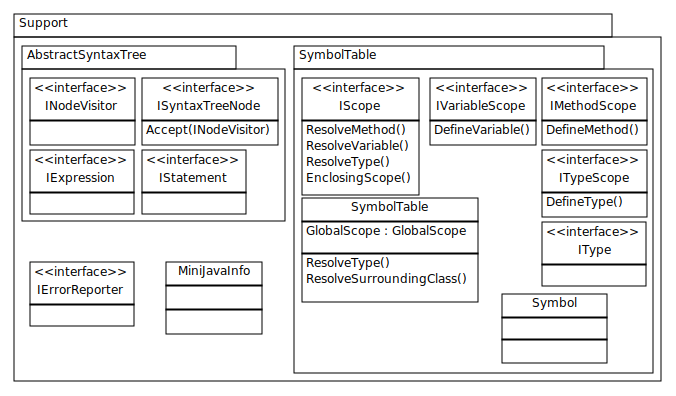
\includegraphics[width=1.0\textwidth]{support.pdf}
\caption{The Support module}
\end{figure}

The support module contains the following parts which are described in more detail below:
\begin{itemize}
\item The abstract syntax tree representation, as described above, and the related INodeVisitor interface.
\item Error handling: an error reporter interface and a basic implementation for it.
\item Static semantic and syntactic information on the language.
\item Symbols, scopes and types
\end{itemize}

The INodeVisitor interface defines Visit methods for all ISyntaxTreeNodes. For some nodes, several entry points are defined. For example, for ClassDeclaration and MethodDeclaration nodes both Visit and Exit methods are provided. In this case, the Visit method is called before any of the nodes children are visited --- the semantic analysis uses this to define and enter the class's or method's scope --- and the Exit method is called after all children have been handled. The latter method is then used e.g. to exit the scope or check that a method's return statements were in order.

More complex visit method groups are defined for IfStatement, WhileStatement and BinaryOperatorExpression which require special treatment in the code generation phase due to the required jump commands and jump labels. In the case of BinaryOperatorExpression, these are used to implement boolean operator short circuiting, which also requires jumps. For example, an IfStatement can be visited after the condition has been evaluated (and before the then branch begins), after the then branch has been evaluated (and before the possible else branch begins) and upon exiting the node (after else branch).

The abstract class NodeVisitorBase provides empty virtual implementations for all methods of the INodeVisitor interface, so each implementing class can just inherit this class and override the methods they need. For clarity, I have drawn all class diagrams so that visitor implementers are marked as implementing INodeVisitor directly, but all of them actually use NodeVisitorBase as their base class.

The IErrorReporter interface provides several methods for reporting and querying for reported errors. E.g. a module can ask whether an error of a certain type (e.g. an error concerning a reference to an unidentified type) has already been reported for a certain syntax tree node. This feature is not extensively utilized by the compiler, but some phases of semantic analysis make use of it.

ErrorLogger provides a basic implementation of the IErrorReporter interface that only logs the errors in a list which can later be e.g. printed by the compiler.

The MiniJavaInfo class holds language information such as listings of keywords, punctuation characters, operators, operator precedences etc. This also includes ''attribute grammar style'' semantic information on MiniJava operators. This is implemented simply as a mapping from operator symbols (actually enum values) to structs that contain the operand type name and the result type name. The semantic analysis phase can utilize this information to check that the operands given for an operator are of the correct type and to deduce the type of expression produced by a particular operator. The class has static methods that can be used to query operator information, check whether a string is a keyword or a built-in type etc.

\begin{figure}[h!]
\centering
\includegraphics[width=0.7\textwidth]{scopes.pdf}
\caption{The interfaces of the Scopes package}
\end{figure}

The Scopes package inside the Support module defines objects that represent lexical and class scopes. The package defines the following interfaces:
\begin{itemize}
    \item IScope, which declares methods for resolving all types of symbols by name. An IScope also has an enclosing scope, which can be null as is in the case of the global scope.
    \item ITypeScope, which represents a scope where 
    \item IMethodScope, which represents a scope where MethodSymbols can be defined. This interface is implemented by ClassScope.
    \item IVariableScope, which represents a scope where VariableSymbols can be defined. This interface is implemented by LocalScope (the scope implementation used for code blocks), MethodScope (the scope used for method bodies, including their parameter lists), ClassScope and ErrorScope.
\end{itemize}

The only difference between MethodScope and LocalScope is that LocalScope can be defined inside any IVariableScope but a MethodScope can only appear inside an IMethodScope. An ErrorScope can be defined inside any IScope. In practice it is used when the symbol table building phase fails to define a method due to a name clash and a ''dummy scope'' is needed to stand in the MethodScope's place.

The IVariableScope interface also provides a method for resolving a local variable. In this case, the search will not proceed to the class level. This is used when a variable is defined in an IVariableScope: the variable can only be defined if a local variable with the same name cannot be found in the scope or one of its enclosing scopes, up to the method scope level. Class variables can still have the same name as a local variable.

\begin{figure}[h!]
\centering
\includegraphics[width=0.7\textwidth]{symbols.pdf}
\caption{The Symbols package}
\end{figure}

The Symbols package defines the abstract class Symbol and the concrete symbol types TypeSymbol, MethodSymbol and VariableSymbol. The Symbol class contains a lot of information: the name of the symbol, the type (IType, described below), the scope it is defined in (an IScope) and also its Declaration in the abstract syntax tree. This can be used to gain access e.g. to a MethodSymbol's MethodDeclaration and its formal parameter declarations, so these do not need to be duplicated in the Symbol object. The most important part of a symbol is the name. TypeSymbols also contain information on the superclass type and can represent either Array or Scalar types.

\begin{figure}[h!]
\centering
\includegraphics[width=0.7\textwidth]{types.pdf}
\caption{The Types package}
\end{figure}

The Types package defines the IType interface that is used to represent types that are not necessarily bound to a type symbol. E.g. the void type is never defined in the symbol table\footnote{There is no reason it could not be defined there as well as any other built-in type, but I have kept it this way to catch programming errors related to handling the void type more easily.}. ScalarType and ArrayType should be self-explanatory: ScalarType represents types that are not arrays (e.g. int) and ArrayType represents types that are (e.g. int[ ]). An ArrayType has a reference to a ScalarType that represents its element type. ErrorType is used when the type of a variable, method return type or an expression cannot be deduced.

ErrorType and VoidType are defined as singletons because I think this is the only way the implementation can make sense semantically: there is only a single type called void, and there is no point in having several instances of ErrorType either. Similarly, there are never several instances of the ScalarType class with the same type name, nor are there several instances of the ArrayType class with the same element type. This is enforced by having ScalarType and ArrayType instances be created only by the static factory methods MakeArrayTypeSymbol and MakeScalarTypeSymbol in the TypeSymbol class. These symbols cannot be defined in the global scope more than once.

The IType interface defines only a single method: IsAssignableTo(IType other). This is implemented by all type classes in such a way, that any type is assignable to ErrorType and ErrorType is assignable to any other type. This helps avoid some special cases when handling ErrorTypes in the semantic analysis phase.

The rules of assignability are as follows: IType T can be assigned to another IType E if and only if
\begin{itemize}
    \item T is the ErrorType instance or
    \item E is the ErrorType instance or
    \item T and E are ScalarType instances and T is defined as a subclass of E or
    \item T = E.
\end{itemize}

This implies that ArrayType instances are only compatible if their element types are the same type. Covariance of array types is therefore not allowed. This is consistent with the MiniJava specification that says ''array types are only compatible if they have the same element type''. This is unlike in Java where arrays are covariant. Of course if T and E are ScalarTypes and T is a subclass of E, T can be assigned into an index of an array of type E[ ].

VoidType can never be assigned to any other type. There is never a case where VoidType is legally the left-hand side of an expression and this situation cannot arise in semantic analysis even through recovery processes.

\subsection{Front-end architecture}

The front end module is divided into three sub-modules, one for each major phase of compilation: lexical analysis, syntax analysis and semantic analysis.

\subsubsection{Simplified view of the front end module}

The FrontEnd class implements the whole front end compilation pipeline with the help of the aforementioned sub-modules that implement the different phases of compilation. These submodules are descibed starting in the next section.

\begin{figure}[h!]
\centering
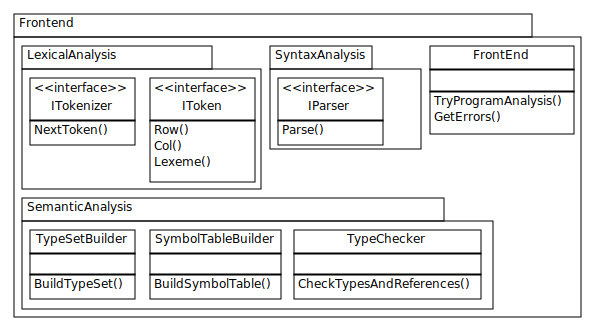
\includegraphics[width=0.7\textwidth]{frontend.pdf}
\caption{The front-end module}
\end{figure}


\subsection{Lexical analysis}

\subsubsection{Module description}

\begin{figure}[h!]
\centering
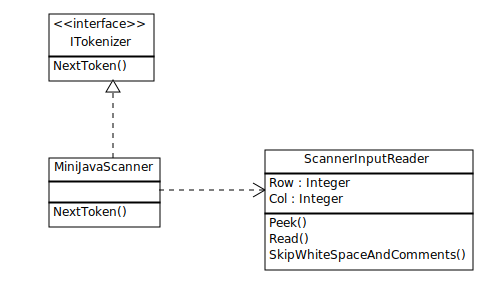
\includegraphics[width=0.7\textwidth]{lexical_analysis.pdf}
\caption{The lexical analysis module}
\end{figure}

The MiniJavaScanner can read input from either a string or a file: it is parameterised with a TextReader (either a StringReader or a StreamReader) for the program code. It offers a very simple interface: it can be asked for the next token in the input stream. At the end of input, a call to NextToken returns an EndOfFile token. If NextToken is still called after that, an OutOfInput exception will be thrown.

In an earlier implementation I had the scanner return EndOfFile indefinitely, but this required special handling in the parser in some places where the parser loops to find e.g. a list of declarations. This way it is more difficult to accidentally construct the parser in such a way that it goes into an infinite loop in some special situations. In practice this exception is handled by the parser.

The MiniJavaScanner passes through the code once when instantiated and builds the queue of tokens. This is done so no one can close the TextReader before the whole token stream is ready. The scanner leaves the TextReader open because it is given as a parameter, so it could in theory still be used by the caller.

Internally, the MiniJavaScanner uses a ScannerInputReader to keep track of the current row and column in the input (for error messages), and skip comments and whitespace. This abstracts away all input handling, so the scanner itself stays cleaner and could easily be replaced by another class that would implement the ITokenizer interface. The only difference between the Peek and Read methods (besides the return type) is that Read consumes the next character before returning it and Peek does not. The ScannerInputReader does not allow peeking several steps forward, although it could. This feature, however, is not required by the MiniJavaScanner.

\subsubsection{Error handling}

The scanner can identify two distinct types of errors:
\begin{enumerate}
\item a multiline comment ended by end of input and
\item an unrecognised token such as characters '\$', '\#' or '@'.
\end{enumerate}

These errors are represented by ErrorToken instances in the token queue. Unlike most other phases of the compiler, the scanner does not throw an exception if it encounters errors like these. The handling of ErrorTokens is left to the caller or the next phase in the pipeline. In practice these errors are handled in the syntax analysis phase.

\subsection{Syntax analysis}

\subsubsection{Module description}

\begin{figure}[h!]
\centering
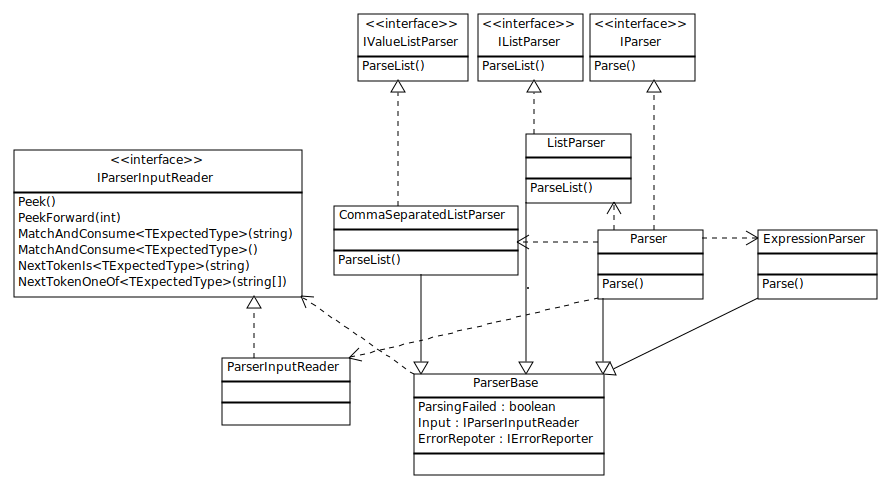
\includegraphics[width=1.0\textwidth]{syntax_analysis.pdf}
\caption{The syntax analysis module}
\end{figure}

This module is used by instantiating a Parser that takes an ITokenizer and an IErrorReporter as inputs. The error reporter is used to report errors and because it is given as a parameter, a single instance can be shared by several classes and across compilation phases. The default implementation for the IErrorReporter logs the errors in a list of ErrorMessages which can then be handled by the higher level module that has access to the reporter instance. A custom implementation could e.g. print error messages into standard output in real time when they are reported.

The Parser offers a TryParse() method that returns a boolean value signaling success (\verb,true,) or failure (\verb,false,). In the latter case the list of errors can be accessed through the error reporter. This is the whole interface needed by the caller.

Internally the parser is split into several parts. The main parser creates a new ExpressionParser instance every time it starts parsing an expression. The ExpressionParser takes care of handling e.g. operator precedences using information provided by the MiniJavaInfo support class. This takes some unnecessary complexity out of the main parser class. In theory, the parser could be further split up into e.g. statement and class parsers.

Additionally, there are two list parsers: a generic ListParser that parses nodes using a parsing function given as a parameter until it encounters the end of file or a specified follow set token. CommaSeparatedListParser does the same but expects the list to use commas as separators. These are used to parse e.g. parameter and argument lists (comma separated) and lists of classes, statements and declarations.

The parser uses a ParserInputReader (or IParserInputReader) that abstracts away input buffering, peeking (even several steps ahead) and matching tokens to a certain token type and possibly content. The parser can e.g. ask the input reader to check that the next token is a PunctuationToken that has the lexeme '\{', and if so, consume it, cast it to the right type and return it. The Consume method of the ParserInputReader is used every time a token is consumed. If the token consumed is an ErrorToken, the ParserInputReader uses the IErrorReporter to report the lexical error. This way all lexical errors get reported, even if those tokens are passed by in a recovery routine.

\subsubsection{Error handling}

The syntax analysis phase can encounter two types of errors:
\begin{enumerate}
\item lexical errors in the form of ErrorTokens from the ITokenizer token queue
\item syntax errors: a token other than what was expected is encountered.
\end{enumerate}

Both types of errors are reported using the IErrorReporter. When an error is encountered, the parser attempts recovery based on reading tokens until one in the follow set is encountered or the end of file is reached. This does not always work terribly well. E.g. if a semicolon is missing from a statement, the recovery routine tries to parse until the next semicolon, because parsing failed while a statement was being parsed. If that statement was the last one in that class, the recovery can end up in the next class. There would be much room for improvement in the parser's recovery routines.

Expression recovery is especially problematic since the follow set for expressions combined is large. Some of these problems could possibly be avoided by careful parameterisation of the recovery routines depending on the exact place where a parse error happened but this would make the parser quite a bit more complex and I am not sure whether the exception based error handling technique used in the current implementation is easily compatible with these kinds of strategies. In a real compiler this could not be allowed, but the parser implementation would probably require some redesign to get a really working implementation.

For many common kinds of syntax errors this basic strategy works fine but some pathological cases can cause a (usually minor) stream of uninformative errors following the one actual error\footnote{Examples with explanations can be found in the recovery test code.}.

For example, when recovering from term parsing, the problem is that the follow set for terms includes e.g. the symbols \verb,[, and \verb,], (used in indexing an array) as well as \verb,),, but these symbols can also appear as a part of a term, e.g. in instance creation expressions (\verb,new int[expr], or \verb,new A(),). As an example, the erroneous code \verb,foo = new int();, will result in two errors: one concerning the symbol \verb,(, when \verb,[, was expected, and one concerning the symbol \verb,),, because recovery assumes that this symbol is already outside the expression and fails to disregard it. However, mostly the recovery strategies appear pretty well-behaved.

If no errors are found, parsing ends with the EndOfFile token being consumed, the root node of the abstract syntax tree is assigned into the output parameter and the return value is \verb,true,. If any errors (lexical or syntactic) have been found, the TryParse method returns \verb,false,.

If syntax analysis fails, the front end module will not continue compilation into the semantic analysis phase. In my experience experimenting with Java, the actual Java compiler is similarly rigid and does not do semantic analysis if syntax analysis fails.\footnote{By including several different semantic errors in the same project one can even discern that semantic analysis is probably divided into clear phases in the Java compiler. Often certain semantic errors cause other types of semantic errors to not be reported at all. A similar approach is taken in this implementation, though I have attempted to make the error recovery in the semantic analysis phase as good as possible.}

\subsection{Semantic analysis}

\subsubsection{Module description}

\begin{figure}[h!]
\centering
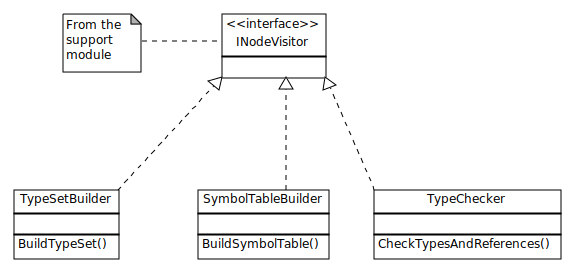
\includegraphics[width=0.8\textwidth]{semantic_analysis.pdf}
\caption{The semantic analysis module. The two-way composition lines mean that one of the classes is defined as a private nested class of the other class and holds a reference to the parent class. E.g. ReferenceChecker is a private nested class of SemanticsChecker. SemanticsChecker creates a ReferenceChecker and a TypeChecker and gives itself as a parameter to these classes constructors.} \label{fig:semantic_analysis}
\end{figure}

The semantic analysis module is implemented by two classes that are run in succession, each producing input for the next phase. Each internal phase passes once through the abstract syntax tree. The phases are:

\begin{enumerate}
\item Building the symbol table (implemented by SymbolTableBuilder).
\item Checking types and the validity of references (implemented by TypeChecker).
\end{enumerate}

\subsubsection{Building the symbol table}

TypeSetBuilder, a nested private class of the SymbolTableBuilder class, collects all the user defined types (class names) in the program and reports name clashes using an IErrorReporter, again given as a parameter to the constructor. The TypeSetBuilder checks clashes with both user-defined and built-in types, although the latter should never happen since having a keyword appear in the place of an identifier should have resulted in a syntax error. If any name clashes are found, the BuildTypeSet method returns false.

TypeSetBuilder used to be a separate module (and class) but is now incorporated as a nested class into the SymbolTableBuilder. Still, if the building of the type set fails, the compiler will not continue even into the rest of the symbol table building phase. This is consistent with the behavior of the actual Java compiler. E.g. the following code compiled with the Java compiler will only result in an error about duplicate classes (\verb,SomeClass,) but will not detect the duplicate method symbol definition or the reference to an unknown type A\footnote{I discovered this by testing programs like these with the Java compiler. Interestingly some IDEs like IntelliJ IDEA \emph{do} detect all of these errors in real time while editing the source even though the compiler does not.}:
\begin{verbatim}
public class SomeClass { }

public class SomeClass { // defined in another file...
  public int foo()
  {
    A a; // unknown type is not detected!
    return 0;
  }

  public int foo() // duplicate method declaration is not detected!
  {
    return 0;
  }
}
\end{verbatim}

The types collected by the TypeSetBuilder as well as all built-in types (int and boolean but not void\footnote{See section \ref{support} for discussion on why the void type is not defined in the symbol table/global scope.}) are defined in the global scope as the first step. The result of this phase is a decoration of the syntax tree with the following information:

\begin{itemize}
    \item Each ISyntaxTreeNode receives a scope. For class and method declarations as well as block scopes this is the scope they define themselves. For all other nodes this is the scope they are defined in.
    \item MethodSymbols and VariableSymbols are defined in the correct scopes.
    \item All TypeSymbols are defined in the global scope.
    \item MethodDeclarations and VariableDeclarations have a Type (or ErrorType if it could not be resolved).
\end{itemize}

The different types of Symbols are described in the Support module section.

Several types of errors can be detected in this phase:
\begin{enumerate}
    \item A symbol definition failure occurs. The rules are detailed below.
    \item A variable or method with an unknown type is declared.
    \item A variable of type void is declared.
    \item A variable or method of type void[ ] is declared.
    \item A class is declared to be derived from an unknown type.
    \item A class depends on itself through the inheritance hierarchy (cyclic inheritance).
\end{enumerate}

The rules of when symbols can and cannot be declared are the following:
\begin{itemize}
    \item A type symbol named A can only be declared if the global scope does not already contain a type symbol with name A.
    \item A variable symbol named A on the class level (a field) can only be declared if the class level scope does not already contain a variable symbol named A. A superclass scope is, of course, allowed to declare a variable with the same name, 
    \item A method symbol named A can only be declared if the class level scope does not already contain a method symbol named A. A superclass scope can contain a method symbol with the same name because overriding is allowed.
    \item A variable symbol named A inside a local scope (an anonymous block) or a method scope can only be declared if the same local/method scope or any of its surrounding local/method scopes does not contain a variable symbol named A. Note: a class field name can be reused as a local variable name or formal parameter name inside a method scope \emph{but} this makes it impossible to refer to the class field from inside that local/method scope because the MiniJava grammar does not allow the use of the \verb,this, keyword when referring to a variable --- it can only be used in method invocations (or when referring to the \verb,length, field of an array) and by itself.
\end{itemize}

Same types of symbols from surrounding scopes can be hidden by symbols with the same name, and the same scope can contain e.g. a variable and a method with the same name, so these cases will not result in an error. If an attempt to define a method fails due to a name clash, an ErrorScope is instantiated to stand in place of the IMethodScope object that would normally be created, so checks can continue. This is the only recovery strategy required in this phase.

Cyclic inheritance and multiple declarations of the same typename are treated as a fatal errors. If these errors occur, semantic analysis cannot continue. However, other types of errors can be recovered from and the compiler can continue into the type checking phase. This phase returns an ExitCode enum value (defined inside SymbolTableBuilder) instead of a boolean value. If a fatal error is encountered (cyclic inheritance or type name clashes), the return value is ExitCode.FatalError. If the error is non-fatal, the return value is ExitCode.NonFatalError and otherwise ExitCode.Success.

\subsubsection{Checking types and the validity of references}

This phase is implemented by the SemanticsChecker class. It produces no output in addition to possible errors, again reported using an IErrorReporter instance. The boolean return value of the RunCheck method signals success (\verb,true,) or failure (\verb,false,).

Internally the phase is divided into two passes through the abstract syntax tree. The first pass (implemented by the ReferenceChecker class) checks references and decorates the tree with type information. The second pass (implemented by the TypeChecker class) performs type checks. Both types of checks could be accomplished in a single pass but this separation of concerns makes the implementation easier to follow. Both classes define a RunCheck method that returns a boolean value indicating success or failure similar to the parent class that utilizes them. Both passes are always run regardless of errors detected in the first pass.

I originally intended to implement checks for references to uninitialized variables but in the end had to leave these checks out due to the rather complicated nature of definite assignment analysis and time constraints.\footnote{E.g. Nicu G. Fruja's article on such checks in C\# describes an approach that would be usable here. The article, \emph{The Correctness of the Definite Assignment Analysis in C\#}, can be found at \url{http://www.jot.fm/issues/issue_2004_10/article2/article2.pdf}.} If implemented, this could be done as an additional pass in the semantic analysis phase.

Because definite assignment is not implemented, local variables are treated like class fields when it comes to initialization: \textbf{int} variables are initialized to 0, \textbf{boolean} variables are initialized to \textbf{false} and reference type variables are initialized to \textbf{null}\footnote{This is actually done by default by the CLR.}. Attempts to call methods on uninitialized reference type variables will, of course, result in a NullReferenceException being thrown by CLR at runtime.

This phase can detect the following types of errors:
\begin{enumerate}
\item A method overloads a method in its superclass. Mini-Java allows only overriding, not overloading.
\item If a method overrides a superclass method, the declared return types of the methods are checked. The return types must be exactly the same or an error is reported. Originally I intended to implement covariant return types similarly to the Java specification\footnote{\url{http://docs.oracle.com/javase/specs/jls/se7/html/jls-8.html\#jls-8.4.5}} but as it turns out, the CLR does not natively support return type covariance, which --- according to Eric Lippert\footnote{See Eric Lippert's post at \\ \url{http://stackoverflow.com/questions/5709034/does-c-sharp-support-return-type-covariance/5709191\#5709191}} --- is the reason C$^\sharp$ does not implement return type covariance either. I have therefore also decided to disallow return type covariance in MiniJava.
\item The arguments to built-in functions or operators (or something similar) are of the wrong type. A ''type grammar'' (attribute grammar style) for operator type checks is defined in the MiniJavaInfo class. Examples of these type requirements are:
\begin{itemize}
\item A print statement requires a single int argument.
\item The argument to an assert statement and the conditional expressions in \verb,if, and \verb,while, statements need to be boolean values.
\item Arithmetic operators and comparison operators require two int arguments.
\item Logical binary operators require two boolean arguments and the unary not operator '!' a single boolean argument.
\item Array sizes and indexing expressions must be int values.
\item The equals operator ('==') accepts any type but both sides must be compatible with each other. Int, boolean and array types require that the other operand is of the same type. For user defined types subtypes are also allowed.
\end{itemize}
\item An attempt is made to index into a variable that is not an array.
\item The left-hand side of an assignment statement is not an L-value. In Mini-Java this means that the left-hand side must be either a reference to a variable (VariableReferenceExpression) or an array element (ArrayIndexingExpression).
\item The assigned value in an assignment statement is not compatible with the type of the L-value it is assigned to. The rules are detailed below this error type list.
\item A method invoked for a user defined type cannot be found.
\item A method is invoked for a built-in type or an array.\footnote{Note: internally the compiler treats the length property of arrays as a method invocation to avoid having to define it as a special case, because it is the only public field in MiniJava. This is the only ''method invocation'' allowed for arrays.}
\item A method is invoked with the wrong number of arguments.
\item A wrong type of argument is passed to a method invocation. Type checks for method invocations follow the same rules as type checks for assignment statements, as detailed below.
\item An integer literal is too large to be represented by a 32-bit integer type, which is the only built-in numeric type in Mini-Java.
\item A reference is made to a variable that cannot be found or a local variable that is in the same scope but has not been introduced yet.
\item A \textbf{void} method has return statements. Empty return statements are not defined in the Mini-Java specification, so this is not allowed.
\item At least some paths in a non-\textbf{void} method do not return a value.
\item Return statements return values of a type different from the one declared in the method signature. Covariance is allowed, so subtypes of the declared type can be returned.
\item An instance creation expression refers to a type name that cannot be found or is an attempt to create a \textbf{void} array (this is allowed by the grammar). Note: an attempt to instantiate a built-in type using a ''new'' expression is detected already in the parsing phase.
\item A static method cannot be called. The only static method in Mini-Java is the main method. In my implementation, calls to the main method have been prevented. I did not see the reason to implement such a feature since there is no use for calling the main method from inside the program, though the MiniJava specification is unclear on whether this should be allowed.
\end{enumerate}

The rules for assignment type checking are as follows:
\begin{itemize}
\item An argument of type void cannot be assigned to any L-value.
\item If the L-value is a built-in type, the assigned value must be of the same type. E.g. an element of an int array has type int, so that is the only type of value that can be assigned to it.
\item If the L-value is an array, the assigned value must also be an array and have the same element type. Unlike in Java, covariance of reference types is not allowed here according to the specification given on the course web site (or appendix B).
\item If the L-value is a user defined (reference) type, the assigned value must be the of the same type or a type derived from it.
\end{itemize}

The same rules apply when checking method invocation argument types: just substitute ''formal parameter'' for ''L-value'' in the rules above.

Internally, a type is anything that implements the IType interface. The IType interface requires that the implementer implements a method IsAssignableTo(IType other). BuiltInTypeSymbol and UserDefinedTypeSymbol (SimpleTypeSymbols) both implement this interface. In addition, there are non-Symbol types: MiniJavaArrayType that is parameterised with a SimpleTypeSymbol (multidimensional arrays are not allowed) and the singleton type VoidType that represents the void return type for methods.

Recovery from errors is needed when the type of an expression cannot be resolved. As mentioned before, the abstract syntax tree is decorated with type information, so for unresolved types the singleton class ErrorType is used. When a method, variable or the type of an instance creation expression cannot be resolved or a non-array variable is indexed, the ErrorType singleton is marked as the type of that syntax tree node.

Every IType is required to implement its IsAssignableTo method in such a way that everything appears to be assignable to an ErrorType -- even the void return type. Similarly, ErrorType is assignable to every other type as well as itself. This way unnecessary type errors related to unresolved types are avoided without having to explicitly check for the ErrorType at every turn. E.g. a program with the lines \verb,A foo; foo = new B();, where \verb,B, cannot be resolved results in an error saying that symbol B could not be resolved but not an error saying that an ErrorType cannot be assigned to a variable of type A.

\subsection{The back-end}

\begin{figure}[h!]
\centering
\includegraphics[width=0.8\textwidth]{backend.pdf}
\caption{The back-end module. See the caption of figure \ref{fig:semantic_analysis} for an explanation on the two-way composition lines.}
\end{figure}

The back-end is a somewhat simpler module than the front-end. This implementation does not do any particular code optimization and the code generated is mostly straightforward.

For code generation, the methods provided by the System.Reflection.Emit namespace are used. This simplifies some tasks like defining assemblies, types and methods while making some things possibly more difficult --- at least for such a simple language as MiniJava. For example, the CodeGenerator must store all System.Reflection.Emit.MethodBuilder objects in a map structure to make method calls possible because it is not possible to query incomplete types for methods by name --- and all user-defined types are incomplete until code generation is complete.

On the other hand, the tools provided by the System.Reflection.Emit namespace take care of things like keeping track of the maximum stack size in a method. The generated assembly is written straight into an \verb,exe, file by the Save method of the AssemblyBuilder class and so does not require running the produced IL code through a separate assembler.

The module is implemented by a single class and its nested INodeVisitor implementations AssemblyGenerator, CodeGenAnalyser and InstructionGenerator. Additionally, InstructionGenerator uses a MethodBodyEmitter instance to emit the actual code of method bodies and to optimize the produced code by performing substitutions on the instruction sequence. These substitutions are described later.

\subsubsection{Additional code analysis.}

CodeGenAnalyser is run prior to any of the other phases. It passes through the tree and decorates it with information required by the code generation phase, such as local indices of local variables and formal parameters.

The CodeGenAnalyser labels LValueExpression nodes (VariableReferenceExpressions and ArrayIndexingExpressions) that are used as the left-hand side of an assignment, so the code generation phase knows when to load the value referred to by the expression and when to just use it as an address. Additionally, it marks whether MethodInvocation nodes are used as stand-alone statements. The InstructionGenerator uses this information to pop unused method return values out of the stack.

The CodeGenAnalyser also detects local variables that are never referenced and takes this into account when calculating indices for locals. The later parts of the back-end will then skip these variables in code generation.\footnote{Opimizations like this can be turned off for e.g. debugging purposes. See running instructions for more information.}

In formal parameter numbering, note that the first parameter in the parameter list of a non-static method is always at index 1 because the implicit \verb,this, reference takes up the index 0.

\subsubsection{Assembly setup}

AssemblyGenerator is used to set up the .NET assembly and and the contained main module. It has the following responsibilities:
\begin{itemize}
    \item It defines the TypeBuilder objects for all user-defined types and stores them in a string to TypeBuilder mapping stored in the parent CodeGenerator object. TypeBuilders need to be stored so they can be finalized after code generation by calling the CreateType() method of the TypeBuilder class.
    \item It defines the ConstructorBuilder objects for all user-defined types. For types that do not have an \verb,extends, declaration, the default constructor that calls the Object class constructor is defined. For types that do have a user-defined superclass, a generic constructor is defined. This constructor does not have a body until it is emitted by the InstructionGenerator. All contructors are stored in a Type to ConstructorBuilder mapping in the parent CodeGenerator object. ConstructorBuilders are needed for generating calls to constructors.
    \item It defines the MethodBuilder objects for all methods inside user-defined classes and stores them in a MethodSymbol to MethodBuilder mapping stored in the parent CodeGenerator object. These need to be stored to make generating calls to methods possible.
    \item It defines the local variables, formal parameters and class fields. Formal parameters and local variables can be referred to by their index, so their builder objects do not need to be stored. FieldBuilders do need to be stored because the ILGenerator.Emit() method requires a FieldBuilder as the second parameter when emitting the opcodes Ldfld (load field) and Stfld (store field). \\
        Local variables are not generated if they were marked as unused by the CodeGenAnalyser.
\end{itemize}

\subsubsection{Instruction generation}

InstructionGenerator generates the actual opcodes of the method and constructor bodies. Method bodies are first generated as a list of OpCode-Object pairs (using Tuple<OpCode?, Object>)\footnote{The OpCode value here is nullable so this listing can also handle label positions in the code. These are stored as a tuple with only the label as the Object value.}. After the complete list of instructions for a single method's body is generated, the InstructionGenerator passes the instruction list to MethodBodyEmitter that performs further optimizations on the instruction list and finally emits the actual opcodes.

Though no code optimization is done, the InstructionGenerator chooses the optimal opcodes for references to variables integer loads. For example, for integer literal loads from 0 to 8, the opcodes \verb,ldc.i4.0, through \verb,ldc.i4.8, are used. For integer literals between 9 and 127 (in the signed byte range), the opcode \verb,ldc.i4.s, is used. For integer literals larger than that, the opcode \verb,ldc.i4, is used. The opcodes for local variable loads (\verb,ldloc.0, through \verb,ldloc.3,, \verb,ldloc.s, for the unsigned byte range, \verb,ldloc, for larger local variable indices) and stores (the corresponding \verb,stloc, codes) and method argument loads and stores (the corresponding \verb,ldarg, codes and \verb,starg.s, for the unsigned byte range and \verb,starg, for larger argument indices) are handled similarly.

For loading boolean literals, the implementation uses \verb,ldc.i4.0, for false and \verb,ldc.i4.1, for true. These are the same opcodes that are used by the C$^\sharp$ compiler. Note that these load integer values represented by four bytes, not a single byte.

In general, for choice in opcodes, I have used the behaviour of the C$^\sharp$ compiler as a reference. I have used the \href{http://ilspy.net/}{ILSpy} .NET decompiler to inspect test programs\footnote{ILSpy formats assembly code in a nicer way than Microsoft's ILDAsm, but it tends to crash when the code is badly malformed, so ILDAsm is sometimes better for debugging problems in code generation.} and figure out how the C$^\sharp$ compiler handles certain situations. As an introduction to the CIL I used the tutorials \href{http://www.codeproject.com/Articles/362076/Understanding-Common-Intermediate-Language-CIL}{Understanding Common Intermediate Language (CIL)} and \href{http://www.codeproject.com/Articles/3778/Introduction-to-IL-Assembly-Language}{Introduction to IL Assembly Language}.

For the most part, code generation for binary operators is straightforward, because the CIL has corresponding opcodes for most of them. These include \verb,add,, \verb,sub,, \verb,mul,, \verb,div,, \verb,clt, (the \verb,<, operator), \verb,cgt, (the \verb,>, operator), \verb,ceq, (the \verb,==, operator) and \verb,rem, (the \verb,%, operator). When the opcode \verb,==, is applied to reference types, the opcode \verb,ceq, handily compares the object references on the evaluation stack, resulting in the correct behavior.

Boolean operators require a bit more effort. The \verb,not, opcode offered by CIL is a bitwise operation. Because the CIL needs to represent boolean values as integers, this cannot be used as a boolean not operation --- the bitwise complement of \textbf{true} would not be \textbf{false}. I have used the same strategy as used by the C$^\sharp$ compiler: emitting an \verb,ldc.i4.0, load opcode and an \verb,ceq, opcode, effectively comparing the boolean value on the stack with \textbf{false}, which results in the same truth table as the boolean not operator.

The CIL does offer (bitwise) opcodes \verb,and, and \verb,or, but in practice these cannot be used because boolean operators need to be short-circuited. This is implemented using jump labels. The implementation of operator short-circuiting is best explained with an example. As an example, the following MiniJava code (a part of the test file \verb,shortcircuit.mjava, that can be found under \verb,testcode/, in the code directory):
\begin{verbatim}
// ... inside the main method
    Test2 a;
    a = new Test2();
    if (!(20 % 2 == 0 && // true
          2 + 2 == 5 &&  // false, short circuits
          a.makeAssertion())) // makeAssertion is never called
    {
      System.out.println(1);
    }

// after the main class:
class Test2
{
  public boolean makeAssertion()
  {
    assert(false);
    return true;
  }
}
\end{verbatim}

The MiniJava compiler produces the following CIL code for the if statement condition (generated without optimizations for branching opcodes):
\begin{verbatim}
// First operand:
IL_0006: ldc.i4.s 20
IL_0008: ldc.i4.2
IL_0009: rem       // 20 % 2
IL_000a: ldc.i4.0
IL_000b: ceq       // == 0, pushes true on the stack
IL_000d: brfalse IL_001d // skip evaluating the other operand if false
                         // consumes the false value on top of the stack!
// Second operand:
IL_0012: ldc.i4.2
IL_0013: ldc.i4.2
IL_0014: add      // 2 + 2
IL_0015: ldc.i4.5
IL_0016: ceq      // == 5, pushes false on the stack
IL_0018: br IL_001e // unconditional branch jumps over the first operand's
                    // short-circuit jump label

IL_001d: ldc.i4.0 // this would re-load false onto the stack if the first operand
                  // had evaluated as false
IL_001e: brfalse IL_002e // jumps over the third operand if one of the
                         // previous operands evaluated as false (as the second
                         // one did)

// Third operand:
IL_0023: ldloc.0  // this code is never reached, so the assertion does not fail
IL_0024: callvirt instance bool Test2::makeAssertion()
IL_0029: br IL_002f // unconditional branch

IL_002e: ldc.i4.0 // re-loads false onto the stack when one of
                  // the earlier operands evaluated as false

IL_002f: ldc.i4.0 // boolean not
IL_0030: ceq
\end{verbatim}

This is almost the same code that the C$^\sharp$ compiler produces for boolean binary operators when the program is compiled without optimizations (i.e. in Debug mode). The difference between logical \verb,and, and \verb,or, operators is mostly that when \verb,and, uses \verb,brfalse, (if the condition is false, jump over other operands), \verb,or, uses \verb,brtrue, (if the condition is true, jump over other operands). Of course the boolean value loaded onto the stack after the jump also differs between the two.

If and while statements also produce similar code to the C$^\sharp$ compiler. Assert statements are in practice implemented similarly to \verb,if, statements. A \verb,brtrue, instruction is generated for jumping over the ''assertion body'' when the condition evaluates as \textbf{true}. The ''body'' prints a message of the format \verb|Exception occurred: AssertionError at <className>.<methodName>| \verb|(<row>,<column>)| which imitates the message produced by Java (although of course Java actually throws an exception). Additionally it produces a call to Environment.Exit with the value 1 as a parameter to indicate failure.

\subsubsection{Optimizations performed by the MethodBodyEmitter}

In addition to optimizing the codes used for integer literal loads as well as argument and local loads and stores, I have also performed optimization on the opcodes used for branching. These are done by the MethodBodyEmitter before emitting the instructions that constitute a method body. It performs the following substitutions:
\begin{itemize}
    \item The opcodes \verb,ldloc.i4.0,, \verb,ceq, (a logical not operation) and either \verb,brtrue, or \verb,brfalse, are replaced with the the opposite comparison branch operator. That is, e.g. the instruction sequence \verb,ldloc.i4.0,, \verb,ceq,, \verb,brtrue, is replaced with a single instruction, \verb,brfalse,. Because the opcodes emitted for a logical not operation are the same as for an integer comparison to zero, this has the slightly peculiar looking effect of also optimizing these integer comparisons in the same way.
    \item The opcodes \verb,ceq, and \verb,brtrue, in sequence are replaced with \verb,beq,.
    \item The opcodes \verb,clt, and \verb,brtrue, in sequence are replaced with \verb,blt,.
    \item The opcodes \verb,cgt, and \verb,brtrue, in sequence are replaced with \verb,bgt,.
    \item The opcodes \verb,clt, and \verb,brfalse, in sequence are replaced with \verb,bge, (branch if greater than or equal to).
    \item The opcodes \verb,cgt, and \verb,brfalse, in sequence are replaced with \verb,ble, (branch if smaller than or equal to).
\end{itemize}

\begin{figure}[h!]
\caption{Code without jump optimization} \label{fig:code_unopt}
\begin{verbatim}
    // ... evaluate a condition ...
    IL_0011: brfalse IL_0034
    // ...
    // an unconditional jump to loop condition:
    IL_0034: br IL_0045
    // begin loop
        // loop body omitted

        // loop condition
        IL_0045: ldloc.1
        IL_0046: ldc.i4.0
        IL_0047: bgt IL_0039
    // end loop
\end{verbatim}
\end{figure}

\begin{figure}[h!]
\caption{Code with jump optimization} \label{fig:code_opt}
\begin{verbatim}
    // ... evaluate a condition ...
    IL_0011: brfalse IL_0045 // jump address has been changed!
    // ...
    // This unconditional jump is still here although
    // there is actually no way to get to it. Deleting it
    // would require analysis of all possible paths through
    // the method body to detect dead code.
    IL_0034: br IL_0045
    // begin loop
        // loop body omitted

        IL_0045: ldloc.1
        IL_0046: ldc.i4.0
        IL_0047: bgt IL_0039
    // end loop
\end{verbatim}
\end{figure}

Instruction sequences with unconditional branching instructions as intermediate jump points are also slightly optimised. If any branch instruction jumps to the label of an unconditional branch instruction (\verb,br,), the first jump instruction's label is replaced with the jump label for the latter instruction. As a result, the code shown in figure \ref{fig:code_unopt} (from an \verb,if, statement with a loop in the \verb,else, branch) becomes the code shown in figure \ref{fig:code_opt}.

The usual jump after a \verb,then, branch in an \verb,if, statement is omitted (already by InstructionGenerator) if the \verb,if, statement has no \verb,else, branch.

\subsection{Shortcomings and potential points of improvement}

Most of these points have already been mentioned, but this part gives a brief summary.

\subsubsection{Recovery strategies}

As far as recovery strategies go, there is probably almost infinite room for improvement. For example, the symbol table building phase could probably pretty easily be made to recover from multiple declarations of the same typename to check for other symbol declaration errors.

However, as said before, I have used the behavior of the actual Java compiler as a guideline for the recovery implementation. The Java compiler does not appear to recover from this situation either. I would guess that this has to do with the fact that recovery over many compilation phases increases the complexity of required tests quite a lot.

\subsubsection{Unimplemented semantic checks}

Some slightly more complicated checks in the semantic analysis phase were left out of this implementation. These include definite assignment checks and unreachable code checks. Both would cause a compile-time error in Java. Neither of these has an effect on the semantics of a program, so I did not implement them due to a lack of time. As mentioned earlier, the CLR default-initializes local variables similarly to instance fields, so local int variables are initialized to 0, local boolean variables to false and local reference type variables to \textbf{null}.

Both of these checks could be implemented as an additional pass in the semantic analysis phase.

\subsubsection{Code optimization}

Obviously code optimization was left out because it was not required in the assignment.

Simple code optimizations that could be implemented include at least the following:
\begin{itemize}
    \item An additional pass in the code generation phase could replace calculations made with literals with a single literal expression (e.g. \verb,42 % 2, could be replaced with \verb,0, or \verb,42 % 2 == 0, with \verb,true,).
    \item Removal of code that does nothing, for example calls to methods with empty bodies, or \verb,if, or \verb,while, statements with empty bodies. This could only be done in rather simple cases, because e.g. a method call parameter or \verb,if, or \verb,while, statement conditions can have side effects.
    \item Methods that are never called could be skipped in code generation because MiniJava programs will definitely not be dynamically linked with any external code that could call these methods...
    \item Currently the code generator marks all user-defined methods (other than main) as virtual and calls them with the \verb,callvirt, instruction to enable overriding. This could be optimized by finding out which methods are actually overridden and marking those methods as virtual, while keeping other methods non-virtual and calling them with the \verb,call, instruction.
\end{itemize}

\subsubsection{Checks in the code generation phase}

The code generation phase does not check that the number of local variables or formal parameters does not exceed the maximum number allowed. In .NET, there can be a maximum of System.UInt16.MaxValue = 65535 local variables or formal parameters in a method, including the \verb,this, reference in non-static methods. For a reference, see e.g. \url{http://msdn.microsoft.com/en-us/library/system.reflection.emit.opcodes.ldloc.aspx} for the local variable case. Documentation for opcodes \verb,starg, or \verb,ldarg, does not mention a limit, but these opcodes also take an UInt16 as a parameter, so it would be reasonable to assume that this is the limit.

In practice, I doubt anyone would define this many local variables or parameters inside a method, and the check would be practically trivial to implement in the pre-code-generation analysis phase implemented by CodeGenAnalyser. This would require giving the back-end component the ability to report errors, which is does not currently have, although it would be simple to add.

\section{Testing}

All modules have been tested using the NUnit test library with a code coverage of nearly 100\%. Mostly trivial parts have been left untested. In practice especially error recovery tests for combinations of errors probably miss some cases, but these are difficult tests to write in general, because the possibilities for different combinations of errors are almost limitless. Some parts of the program have been unit-tested but most parts should be involved in integration tests as well.

I have attempted to test the recovery paths in the parsing and semantic analysis phases as well as I have been able to, but thorough testing of recovery routines is difficult due to the large number of different paths through recursive parsers and visitors. These are probably the most likely source of bugs.

If bugs remain in the system (as some almost certainly do), the best case scenario is that they will only lead to bad error messages in some cases. The worst case scenario for the parser is being stuck in an infinite loop when attempting to recover. During development I have found a few such bugs and managed to fix them but I would not be very surprised if some untested recovery path still led to such a problem, since the parser is rather difficult to reason about.

At the moment, however, I do not know of any existing bugs in the compiler.

The code generation part is tested by running test programs through the whole compilation pipeline and checking the produced programs' output against a reference result. All programs are also verified with the PEVerify tool and its output is also automatically tested. The actual instruction generation is not tested (that is, the programs are not disassembled to automatically inspect the instructions generated), but I have checked the IL code generated for all test programs manually and corrected all of the bugs that I have found.

The directory \verb,testcode/, under the main code directory contains example programs that can be compiled with MiniJavaCompiler.exe and verified with PEVerify. These are also used in the automated code generation tests.

Note that the code generation tests require a path to the PEVerify.exe program. This can be set by editing the class variable PEVerifyPath in CodeGenTest.cs, but at least on the department machines I tested, the path to PEVerify.exe was the same as on my computer (the default path), so these should run fine without any edits.

On department systems with Visual Studio 2012, NUnit can be installed through the package manager, to make the test project compile. Installing the \href{http://nunit.org/index.php?p=vsTestAdapter&r=2.6.1}{NUnit test adapter} enables these tests to be run using the test menu/test explorer of Visual Studio. If the test adapter cannot be found using the built-in package manager, it can also be \href{http://visualstudiogallery.msdn.microsoft.com/6ab922d0-21c0-4f06-ab5f-4ecd1fe7175d}{downloaded from here}.

\section{Building and running the compiler}

The easiest way to build the compiler solution is opening it in Visual Studio and building it in Release mode to disable assertions and to get optimised code. Note that the test project requires NUnit to build successfully, as described in the previous section.

After this the resulting \verb,MiniJavaCompiler.exe, under \verb,bin\Release, can be run by giving it the path to the source file as a parameter (and optionally a path to an output file): \verb,./MiniJavaCompiler.exe path/to/source/file [path/to/output/file],.

An additional parameter \verb,-no-opt, can be given as an optional \emph{first}\footnote{The compiler is strict about the ordering of its parameters.} parameter to the compiler to disable optimizations in the code generation phase. This will generate code for unused variables and leave jump instructions unoptimized.

Running the compiler without any arguments or with the input file name missing prints out the usage instructions as detailed above.

The solution is targeted for .NET 4.5 to get access to System.Tuple, so it probably cannot be run on e.g. the department Windows server that still runs Visual Studio 2010.

The program code and the \LaTeX{} sources for this documentation are also available on \href{https://github.com/Lateks/MiniJavaCompiler}{my GitHub account page} where the repository can be cloned.


\appendix
\section{Project definition}

\includegraphics[width=1.0\textwidth,page=1]{project.pdf}
\includegraphics[width=1.0\textwidth,page=2]{project.pdf}

\section{Mini-Java specification}

\includegraphics[width=1.0\textwidth,page=1]{spec.pdf}
\includegraphics[width=1.0\textwidth,page=2]{spec.pdf}
\includegraphics[width=1.0\textwidth,page=3]{spec.pdf}
\end{document}
